\scanpage{155}
% archive foliation: 154
Conditions équivalentes:
\[
\left\{\begin{array}{ll}
a)&\mathrm{Pic}_{C/k}^0\text{ est abélien}\\
b)&\text{les }\mu_\alpha=0\text{ i.e. tous les pts doubles sont ordinaires,}\\
&\uuline{\text{et}}\quad b_1=0\quad[\text{En particulier les }C_i\text{ sont non singuliers}]
\end{array}\right.
\]
Conditions équivalentes
\[
\left\{\begin{array}{ll}
a)&\mathrm{Pic}_{C/k}^0\text{ n'a pas de composante additive}\\
b)&\deleted{\text{Donc}}\ \forall\alpha,\text{ on a }\mu_\alpha=\mu'_\alpha\\
&\text{i.e. le recollement est trivial.}
\end{array}\right.
\]
\figure{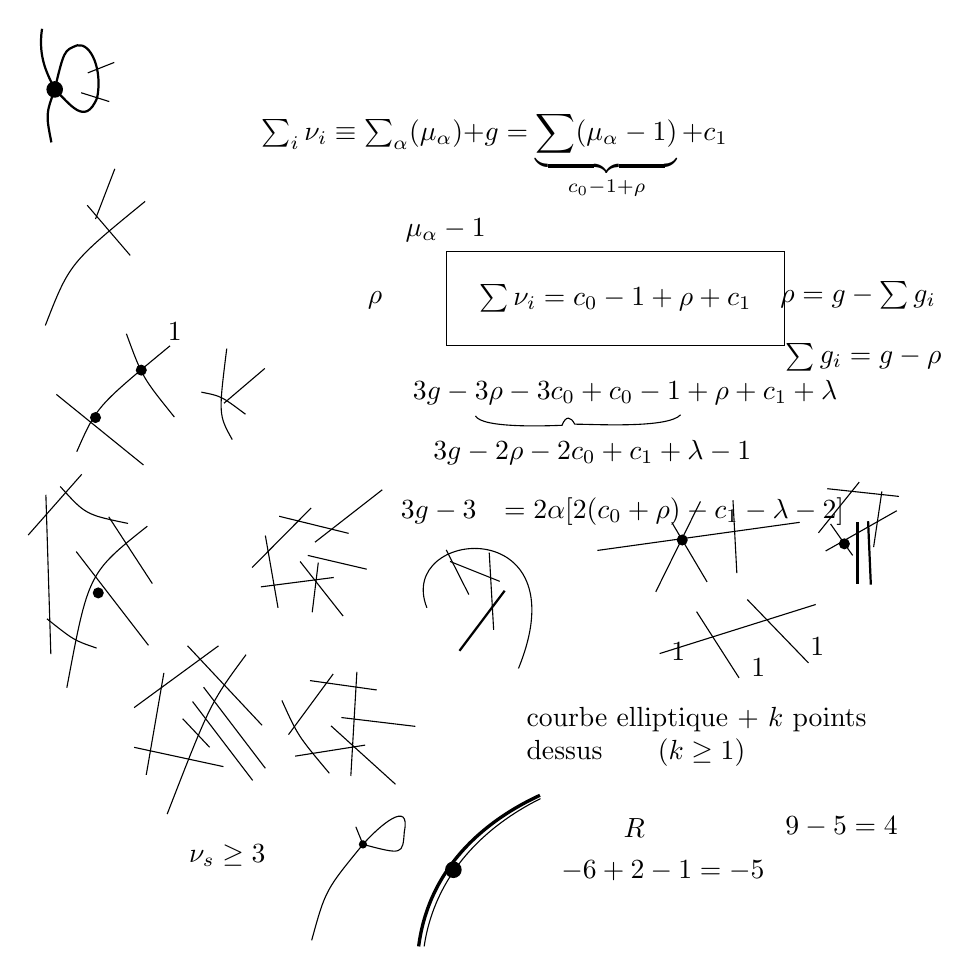
\begin{tikzpicture}[x=.007cm,y=-.007cm]
\draw[thick] (80,515)..controls (72,570) and (92,600)..(103,625)..controls (130,650) and (158,694)..(180,640)..controls (190,590) and (169,540)..(144,545)..controls (120,554)..(103,625)..controls (87,670)..(97,721);
\fill (103,625) circle (3pt);\draw (163,595)--(211,576);\draw (151,631)--(202,647);
\draw (86,1053)..controls (130,940)..(267,828);\draw (162,835)--(240,926);\draw (177,860)--(212,769);
\node[anchor=west] at (460,745) {$\sum_i\nu_i\equiv\sum_\alpha(\mu_\alpha)\deleted{\unsure{+g}}=\underbrace{\sum(\mu_\alpha-1)}_{c_0-1+\rho}+c_1$};
\node at (812,881) {$\mu_\alpha-1$};
\node at (684,1008) {$\deleted{\unsure{\rho}}$};
\node[draw,inner sep=12pt] at (1120,1004) {$\sum\nu_i=c_0-1+\rho+c_1$};
\node at (1560,998) {$\rho=g-\sum g_i$};\node at (1570,1110) {$\sum g_i=g-\rho$};
\draw (143,1282)..controls (179,1200)..(312,1090);\draw (106,1178)--(264,1306);\draw (233,1068)..controls (262,1147)..(320,1219);\fill (177,1220) circle (2pt);\fill (260,1134) circle (2pt);\node at (321,1065) {$1$};
\draw (415,1095)..controls (400,1215)..(425,1260);\draw (369,1174)..controls (405,1181)..(449,1214);\draw (410,1194)--(484,1131);
\node[anchor=west] at (735,1175) {$3g-3\rho-\unsure{3c_0}+\deleted{c_0}-1+\rho+c_1+\lambda$};
\draw (866,1217)..controls (878,1240) and (998,1235)..(1023,1234)..controls (1030,1216) and (1039,1218)..(1046,1232)..controls (1082,1232) and (1215,1240)..(1238,1215);
\node[anchor=west] at (772,1284) {$3g-2\rho-2c_0+c_1+\lambda-1$};
\node[anchor=west] at (713,1390) {$3g-3\quad\deleted{\unsure{=2\alpha}}[2(c_0+\rho)-c_1-\lambda-2]$};
\draw (55,1433)--(152,1323);\draw (113,1345)..controls (159,1396)..(236,1412);\draw (87,1360)--(96,1649);\draw (201,1400)--(280,1521);\draw (271,1417)..controls (164,1502)..(125,1710);\draw (142,1463)--(273,1633);\draw (89,1585)..controls (138,1624)..(179,1638);\fill (182,1538) circle (2pt);
\draw (461,1492)--(568,1384);\draw (510,1399)--(636,1430);\draw (575,1446)--(697,1351);\draw (485,1434)--(508,1565);\draw (562,1470)--(669,1495);\draw (477,1527)--(609,1510);\draw (548,1481)--(626,1580);\draw (581,1483)--(570,1573);
\draw (813,1460)--(854,1541);\draw (820,1481)--(910,1517);\draw (891,1465)--(899,1605);\draw[thick] (837,1643)--(919,1534);\draw (778,1565)..controls (720,1420) and (1060,1390)..(944,1675);
\draw (1087,1461)--(1454,1410);\draw (1193,1536)--(1274,1372);\draw (1222,1410)--(1286,1518);\draw (1333,1370)--(1340,1502);\fill (1241,1442) circle (2pt);
\draw (1488,1429)--(1562,1337);\draw (1504,1349)--(1634,1363);\draw (1510,1413)--(1550,1470);\draw (1501,1462)--(1630,1389);\draw (1603,1354)--(1588,1455);\draw[very thick] (1559,1410)--(1559,1522);\draw[thick] (1578,1408)--(1583,1523);\fill (1535,1449) circle (2pt);
\draw (1200,1648)--(1483,1559);\draw (1267,1572)--(1344,1692);\draw (1359,1550)--(1470,1665);\node at (1234,1645) {$1$};\node at (1379,1674) {$1$};\node at (1486,1636) {$1$};
\draw (247,1746)--(400,1634);\draw (301,1683)--(269,1868);\draw (344,1634)--(479,1778);\draw (450,1650)..controls (385,1738)..(307,1939);\draw (373,1709)--(485,1856);\draw (353,1735)--(462,1878);\draw (335,1766)--(384,1818);\draw (247,1818)--(409,1853);
\draw (527,1795)--(608,1685);\draw (566,1697)--(687,1714);\draw (651,1681)--(640,1870);\draw (515,1733)..controls (544,1797)..(601,1865);\draw (623,1764)--(757,1780);\draw (539,1834)--(666,1814);\draw (604,1779)--(721,1885);
\node[align=left] at (1267,1799) {courbe elliptique $+\ k$ points\\dessus\qquad$(k\geq1)$};
\node at (416,2015) {$\nu_s\geq3$};
\draw (569,2168)..controls (594,2077)..(662,1994)..controls (692,1960) and (749,1911)..(737,1971)..controls (734,2013)..(662,1994)--(649,1962);\fill (662,1994) circle (1.5pt);
\draw[very thick] (763,2179)..controls (781,2039) and (879,1953)..(983,1905);\draw (773,2179)..controls (792,2050) and (881,1962)..(984,1911);\fill (826,2040) circle (3pt);
\node at (1154,1965) {$\unsure{\mathbb R}$};\node at (1530,1962) {$9-5=4$};\node at (1206,2041) {$-6+2-1=-5$};
\end{tikzpicture}}

